\PassOptionsToPackage{x11names}{xcolor}
\documentclass{beamer}

\beamertemplatenavigationsymbolsempty

\usepackage{agda}
\usepackage{stmaryrd}
\usepackage{mathtools}
\usepackage{etoolbox}
\usepackage{idris2}
\usepackage{catchfilebetweentags}
\makeatletter

\newrobustcmd*\OrigExecuteMetaData[2][\jobname]{%
\CatchFileBetweenTags\CatchFBT@tok{#1}{#2}%
\global\expandafter\CatchFBT@tok\expandafter{%
\expandafter}\the\CatchFBT@tok
}%\OrigExecuteMetaData

\newrobustcmd*\ChkExecuteMetaData[2][\jobname]{%
\CatchFileBetweenTags\CatchFBT@tok{#1}{#2}%
\edef\mytokens{\detokenize\expandafter{\the\CatchFBT@tok}}
\ifx\mytokens\empty\PackageError{catchfilebetweentags}{the tag #2 is not found\MessageBreak in file #1 \MessageBreak called from \jobname.tex}{use a different tag}\fi%
}%\ChkExecuteMetaData

\renewrobustcmd*\ExecuteMetaData[2][\jobname]{%
\ChkExecuteMetaData[#1]{#2}%
\OrigExecuteMetaData[#1]{#2}%
}

\makeatother

\usepackage{hyperref}
\usepackage{cleveref}
\usepackage{bytefield}

%\usepackage{fullpage}

\usepackage{todonotes}
\setuptodonotes{inline}

\usepackage{listings}

\lstset{ %
  language=C,
  numbers=left,
  numberstyle=\tiny,
  stepnumber=1,
  numbersep=5pt,
  breaklines=true,
  otherkeywords={uint8_t},
}

\usepackage{pgfplots}
\pgfplotsset{compat=1.16, width=\textwidth}

%%%%%%%%%%%%% SUBMISSION PROCESSES

\newtoggle{BLIND}

\newcommand{\usestt}{\small}

%%%%%%%%%%%%%%%%%%%%%%%%%%%

%%% Languages

\newcommand{\agda}{Agda}
\newcommand{\idris}{Idris~2}

%%% Idris highlighting

\newcommand{\assertTotal}{\IdrisPostulate{assert\KatlaUnderscore{}total}}
\newcommand{\believeMe}{\IdrisPostulate{believe\KatlaUnderscore{}me}}

%%% Data highlighting

\newcommand{\hexadesc}[1]{\texttt{\usestt\IdrisType{#1}}}
\newcommand{\hexadata}[1]{\texttt{\usestt\IdrisData{#1}}}
\newcommand{\hexacons}[1]{\texttt{\usestt\IdrisFunction{#1}}}
\newcommand{\hexaoffset}[1]{\texttt{\usestt{\color{lightgray}#1}}}

\newenvironment{hexdump}{\usestt\medskip\ttfamily\obeyspaces\obeylines\noindent}{\medskip}

%%% Links to supplementary material
\newcommand{\suppfile}[1]{File \texttt{#1}}

%%% Remark environment
\usepackage{amsthm}
\newtheorem{remark}{Idris-ism}


\title{Scoped and Typed Staging by Evaluation}
\author{Guillaume Allais}
\institute{University of Strathclyde}
\date{PLUG \\ November 8$^{th}$ 2023}


\AtBeginSection[]
{
    \begin{frame}
        \frametitle{Table of Contents}
        \tableofcontents[currentsection]
    \end{frame}
}

\begin{document}

\begin{frame}
  \maketitle
\end{frame}

\section{Goals}

\begin{frame}{Different motivations}
Generic programming:

\begin{itemize}
  \item using the language itself
  \item in a type-safe manner
  \item with no abstraction cost
\end{itemize}

\bigskip

Meta programming:

\begin{itemize}
  \item in a richer language
  \item in a type-safe manner
  \item with no abstraction cost
\end{itemize}
\end{frame}

\begin{frame}{An example: the diagonal of a circuit}
  \begin{minipage}{.6\textwidth}
    \ExecuteMetaData[MetaCircuit.tex]{dup}
  \end{minipage}\hfill
  \begin{minipage}{.3\textwidth}
    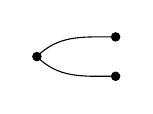
\begin{tikzpicture}
    \draw[fill] (0,.25) circle[radius=1.5pt] node { };

      \draw[fill] (1,0)  circle[radius=1.5pt] node { };
      \draw[fill] (1,.5) circle[radius=1.5pt] node { };

      \draw[-] (0,.25) to [out=-45,in=180] (.95,0);
      \draw[-] (0,.25) to [out=45,in=180] (.95,.5);
    \end{tikzpicture}
  \end{minipage}
  \bigskip

  \ExecuteMetaData[MetaCircuit.tex]{diag}

  \begin{minipage}{.05\textwidth}
    $c \mapsto$
  \end{minipage}
  \begin{minipage}{.375\textwidth}
    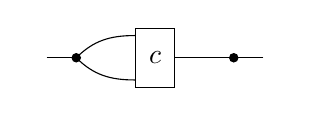
\begin{tikzpicture}

      \coordinate (x) at (0,.25);
      \draw[fill] (x) circle[radius=1.5pt] node {};
      \draw (x)+(-.5,0) node {} edge (x);

      \node[rectangle, draw, minimum height=.75cm, minimum width=.5cm] at (1, .25) (c) {$c$};

      \draw[-] (x) to [out=-45,in=180] ([yshift=.1cm] c.south west);
      \draw[-] (x) to [out=45,in=180] ([yshift=-.1cm] c.north west);

      \coordinate (r) at ([xshift=1cm] c);
      \draw[fill] (r) circle[radius=1.5pt] node {};
      \draw[-] (c.east) to (r);
      \draw (r)+(.5,0) node {} edge (r);
    \end{tikzpicture}
  \end{minipage}

  \bigskip
  \begin{minipage}[t]{.45\textwidth}
    \ExecuteMetaData[MetaCircuit.tex]{not}
  \end{minipage}\hfill
  \begin{minipage}[t]{.45\textwidth}
    \ExecuteMetaData[MetaCircuit.tex]{testNot}
  \end{minipage}
\end{frame}

\section{Refresher: scoped-and-typed syntax}

\begin{frame}{Types and Contexts}

  \ExecuteMetaData[STLC.tex]{type}
  \ExecuteMetaData[STLC.tex]{typevariables}

  \bigskip

  \uncover<2->{\ExecuteMetaData[STLC.tex]{context}}
\end{frame}

\begin{frame}{Convention: Implicit context threading}

\begin{minipage}{.45\textwidth}
  \begin{mathpar}
    \inferrule{Γ ⊢ f : A → B \and Γ ⊢ t : A}{Γ ⊢ f \, t : B} \and
    \inferrule{Γ, x : A ⊢ b : B}{Γ ⊢ λx.b : A → B}
  \end{mathpar}
\end{minipage}\hfill
\begin{minipage}{.45\textwidth}
  \begin{mathpar}
    \inferrule{f : A → B \and t : A}{f \, t : B} \and
    \inferrule{x : A ⊢ b : B}{λx.b : A → B}
  \end{mathpar}
\end{minipage}
\end{frame}

\begin{frame}{Tools: implicit context threading}

  Combinators:

  \begin{minipage}{.3\textwidth}
    \ExecuteMetaData[STLC.tex]{forall}
  \end{minipage}\hfill
  \begin{minipage}{.55\textwidth}
  \uncover<2->{
    \ExecuteMetaData[STLC.tex]{update}}
  \end{minipage}

  \begin{minipage}{.45\textwidth}
  \uncover<3->{
    \ExecuteMetaData[STLC.tex]{arrow}}
  \end{minipage}\hfill
  \begin{minipage}{.45\textwidth}
  \uncover<4->{
    \ExecuteMetaData[STLC.tex]{product}}
  \end{minipage}

  \bigskip

  \uncover<5->{
  Example:

  \begin{AgdaSuppressSpace}
    \ExecuteMetaData[STLC.tex]{swaptype}
    \ExecuteMetaData[STLC.tex]{swaptypenormalised}
  \end{AgdaSuppressSpace}}

\end{frame}

\begin{frame}{Scoped-and-typed De Bruijn indices}
  \ExecuteMetaData[STLC.tex]{var}

  \begin{mathpar}
    \inferrule{ }{x : A ⊢ x :_v A} \and
    \inferrule{x :_v A}{y : B ⊢ x :_v A}
  \end{mathpar}
\end{frame}

\begin{frame}{Scoped-and-typed syntax}
  \ExecuteMetaData[STLC.tex]{termdecl}
\end{frame}

\begin{frame}{Scoped-and-typed syntax: variable}
  \begin{minipage}[t]{.45\textwidth}
    \ExecuteMetaData[STLC.tex]{termvar}
  \end{minipage}\hfill
  \begin{minipage}[t]{.45\textwidth}
  \begin{mathpar}
    \inferrule{x :_v A}{x : A}
  \end{mathpar}
  \end{minipage}
\end{frame}

\begin{frame}{Scoped-and-typed syntax: application}
  \begin{minipage}[t]{.45\textwidth}
    \ExecuteMetaData[STLC.tex]{termapp}
  \end{minipage}\hfill
  \begin{minipage}[t]{.45\textwidth}
  \begin{mathpar}
    \inferrule{f : A → B \and t : A}{f \, t : B}
  \end{mathpar}
  \end{minipage}
\end{frame}


\begin{frame}{Scoped-and-typed syntax: λ-abstraction}
  \begin{minipage}[t]{.45\textwidth}
    \ExecuteMetaData[STLC.tex]{termlam}
  \end{minipage}\hfill
  \begin{minipage}[t]{.45\textwidth}
  \begin{mathpar}
    \inferrule{x : A ⊢ b : B}{λx.b : A → B}
  \end{mathpar}
  \end{minipage}
\end{frame}

\begin{frame}{Scoped-and-typed syntax}
  \ExecuteMetaData[STLC.tex]{term}

  \bigskip

  \ExecuteMetaData[STLC.tex]{id}
\end{frame}

\section{Refresher: scoped-and-typed semantics}

\begin{frame}{What do we want?}
  \ExecuteMetaData[STLC.tex]{evaldecl}
\end{frame}

\begin{frame}{Category of weakenings}
  \ExecuteMetaData[STLC.tex]{ope}

  \bigskip

  \begin{AgdaSuppressSpace}
    \ExecuteMetaData[STLC.tex]{lerefl}
    \ExecuteMetaData[STLC.tex]{letrans}
  \end{AgdaSuppressSpace}
\end{frame}

\begin{frame}{Action of weakenings on syntax}
  \ExecuteMetaData[STLC.tex]{weaken}

  \ExecuteMetaData[STLC.tex]{weakVar}
  \ExecuteMetaData[STLC.tex]{weakTerm}
\end{frame}

\begin{frame}{Model construction: Kripke function spaces}

\ExecuteMetaData[STLC.tex]{box}

\uncover<2->{
\begin{minipage}{.3\textwidth}
  \ExecuteMetaData[STLC.tex]{extract}
\end{minipage}\hfill\begin{minipage}{.6\textwidth}
\ExecuteMetaData[STLC.tex]{duplicate}
\end{minipage}}

\uncover<3->{
\ExecuteMetaData[STLC.tex]{kripke}
\ExecuteMetaData[STLC.tex]{mkbox}
}

\uncover<4->{
\begin{minipage}{.45\textwidth}
  \ExecuteMetaData[STLC.tex]{semapp}
\end{minipage}\hfill\begin{minipage}{.45\textwidth}
\ExecuteMetaData[STLC.tex]{weakKripke}
\end{minipage}}
\end{frame}

\begin{frame}{Model construction: values}
  \ExecuteMetaData[STLC.tex]{value}

  \bigskip

  \ExecuteMetaData[STLC.tex]{weakValue}
\end{frame}

\begin{frame}{Model construction: environments}
  \ExecuteMetaData[STLC.tex]{env}

  \ExecuteMetaData[STLC.tex]{extend}
\end{frame}

\begin{frame}{Model construction: evaluation}
  \begin{AgdaSuppressSpace}
  \ExecuteMetaData[STLC.tex]{eval}
  \end{AgdaSuppressSpace}
\end{frame}


\section{Minimal Intrinsically Typed Two Level Type Theory}

\begin{frame}{Example}
  \ExecuteMetaData[BasicTwoTT.tex]{testid01}
\end{frame}

\begin{frame}{Phases, Stages, and Types}
  \ExecuteMetaData[BasicTwoTT.tex]{phase}
  \uncover<2->{\ExecuteMetaData[BasicTwoTT.tex]{stage}}
  \uncover<3->{\ExecuteMetaData[BasicTwoTT.tex]{types}}
\end{frame}

\begin{frame}{Scoped-and-typed syntax}
  \begin{AgdaSuppressSpace}
    \ExecuteMetaData[BasicTwoTT.tex]{termdecl}

    \medskip
    \uncover<2->{
      \hfill\begin{minipage}{.95\textwidth}
        \ExecuteMetaData[BasicTwoTT.tex]{termstlc}
      \end{minipage}}

    \medskip
    \uncover<3->{
      \hfill\begin{minipage}{.95\textwidth}
        \ExecuteMetaData[BasicTwoTT.tex]{termtwolevel}
      \end{minipage}}
  \end{AgdaSuppressSpace}

  \bigskip

  \uncover<4->{
    \begin{minipage}{.45\textwidth}
      \ExecuteMetaData[BasicTwoTT.tex]{iddyn}
    \end{minipage}\hfill
    \begin{minipage}{.45\textwidth}
      \ExecuteMetaData[BasicTwoTT.tex]{idsta}
    \end{minipage}}
\end{frame}

\begin{frame}{What do we want?}
  \ExecuteMetaData[BasicTwoTT.tex]{evaldecl}
  \ExecuteMetaData[BasicTwoTT.tex]{stagedecl}
\end{frame}

\begin{frame}{Model construction: values}
  \ExecuteMetaData[BasicTwoTT.tex]{model}

  \begin{AgdaSuppressSpace}
    \ExecuteMetaData[BasicTwoTT.tex]{modelstadecl}
    \ExecuteMetaData[BasicTwoTT.tex]{modelsta}
  \end{AgdaSuppressSpace}
\end{frame}

\begin{frame}{Model construction: evaluation}
  \begin{AgdaSuppressSpace}
    \ExecuteMetaData[BasicTwoTT.tex]{evaldecl}
    \ExecuteMetaData[BasicTwoTT.tex]{eval}
  \end{AgdaSuppressSpace}

  \begin{AgdaSuppressSpace}
    \ExecuteMetaData[BasicTwoTT.tex]{bodydecl}
    \ExecuteMetaData[BasicTwoTT.tex]{body}
  \end{AgdaSuppressSpace}
\end{frame}

\begin{frame}{Model construction: evaluation (ctd)}
  \ExecuteMetaData[BasicTwoTT.tex]{app}

  \bigskip

  \uncover<2->{\ExecuteMetaData[BasicTwoTT.tex]{lam}}
\end{frame}

\begin{frame}{Model construction: staging}
  \begin{AgdaSuppressSpace}
    \ExecuteMetaData[BasicTwoTT.tex]{stagefun}
  \end{AgdaSuppressSpace}
\end{frame}

\section{Radically Different Meta and Object Languages}

\begin{frame}{A circuit language}
  \ExecuteMetaData[MetaCircuit.tex]{type}
  \uncover<2->{\ExecuteMetaData[MetaCircuit.tex]{termcircuitnand}}
  \uncover<3->{\ExecuteMetaData[MetaCircuit.tex]{termcircuitpar}}
  \uncover<4->{\ExecuteMetaData[MetaCircuit.tex]{termcircuitseq}}
  \uncover<5->{\ExecuteMetaData[MetaCircuit.tex]{termcircuitmix}}
\end{frame}

\begin{frame}{Wiring examples}

  \begin{minipage}{.6\textwidth}
    \ExecuteMetaData[MetaCircuit.tex]{id2}
  \end{minipage}\hfill
  \begin{minipage}{.3\textwidth}
    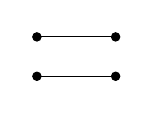
\begin{tikzpicture}
      \draw[fill] (0,0)  circle[radius=1.5pt] node { };
      \draw[fill] (0,.5) circle[radius=1.5pt] node { };

      \draw[fill] (1,0)  circle[radius=1.5pt] node { };
      \draw[fill] (1,.5) circle[radius=1.5pt] node { };

      \draw[-] (0,0)  to [out=0,in=180] (.95,0);
      \draw[-] (0,.5) to [out=0,in=180] (.95,.5);
    \end{tikzpicture}
  \end{minipage}

  \begin{minipage}{.6\textwidth}
    \ExecuteMetaData[MetaCircuit.tex]{swap}
  \end{minipage}\hfill
  \begin{minipage}{.3\textwidth}
    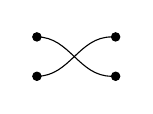
\begin{tikzpicture}
      \draw[fill] (0,0)  circle[radius=1.5pt] node { };
      \draw[fill] (0,.5) circle[radius=1.5pt] node { };

      \draw[fill] (1,0)  circle[radius=1.5pt] node { };
      \draw[fill] (1,.5) circle[radius=1.5pt] node { };

      \draw[-] (0,0)  to [out=0,in=180] (.95,.5);
      \draw[-] (0,.5) to [out=0,in=180] (.95,0);
    \end{tikzpicture}
  \end{minipage}

  \begin{minipage}{.6\textwidth}
    \ExecuteMetaData[MetaCircuit.tex]{dup}
  \end{minipage}\hfill
  \begin{minipage}{.3\textwidth}
    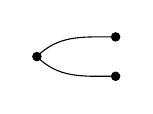
\begin{tikzpicture}
      \draw[fill] (0,.25) circle[radius=1.5pt] node { };

      \draw[fill] (1,0)  circle[radius=1.5pt] node { };
      \draw[fill] (1,.5) circle[radius=1.5pt] node { };

      \draw[-] (0,.25) to [out=-45,in=180] (.95,0);
      \draw[-] (0,.25) to [out=45,in=180] (.95,.5);
    \end{tikzpicture}
  \end{minipage}
  \end{frame}

\begin{frame}{Recovering the usual logic gates}
  \ExecuteMetaData[MetaCircuit.tex]{diag}
  \ExecuteMetaData[MetaCircuit.tex]{not}
  \ExecuteMetaData[MetaCircuit.tex]{and}
  \ExecuteMetaData[MetaCircuit.tex]{or}
\end{frame}

\begin{frame}{Tabulating a function}
  \ExecuteMetaData[MetaCircuit.tex]{tab}


  \medskip
  \begin{minipage}{.05\textwidth}
    $f \mapsto$
  \end{minipage}\hfill
  \begin{minipage}{.8\textwidth}\scalebox{.85}{
    \begin{tikzpicture}{circuit logic US}
      \coordinate (b) at (0,2);
      \draw[fill] (b) circle[radius=1.5pt] node {};
      \draw (b)+(-.5,0) node {$b$} edge (b);

      \coordinate (x) at (0,0);
      \draw[fill] (x) circle[radius=1.5pt] node {};
      \draw (x)+(-.5,0) node {$x$} edge (x);

      \node[rectangle, draw] at (2, 1.5) (f1) {$f\,1$};
      \draw[-] (x) to [out=45, in=180] (f1);

      \node[rectangle, draw] at (2, 0) (f0) {$f\,0$};
      \draw[-] (x) to [out=0, in=180] (f0);

      \draw (4, 0.15) node[and port, scale=.5] (and0) {};
      \draw[-] (f0) [out=0, in=180] to (and0.in 2);

      \draw (4, 1.85) node[and port, scale=.5] (and1) {};
      \draw[-] (b) [out=0, in=180] to (and1.in 1);
      \draw[-] (f1) [out=0, in=180] to (and1.in 2);

      \draw (2, .65) node[not port, scale=.35] (not0) {};
      \draw[-] (b) [out=-45, in=180] to (not0.in 1);
      \draw[-] (not0.out) [out=0, in=180] to (and0.in 1);

      \draw (6, 1) node[or port, scale=.5] (or01) {};
      \draw[-] (and1.out) [out=0, in=180] to (or01.in 1);
      \draw[-] (and0.out) [out=0, in=180] to (or01.in 2);

      \coordinate (tag) at (7,1);
      \draw[fill] (tag) circle[radius=1.5pt] node {};
      \draw (tag)+(.5,0) node {$r$} edge (tag);
      \draw[-] (or01.out) to (tag);

      \draw[dashed] ([xshift=-.25cm, yshift=1cm] x) to ([xshift=.5cm, yshift=1cm] x);
      \draw[dashed] ([xshift=.5cm, yshift=.4cm] b) to ([xshift=.5cm, yshift=-.4cm] x);
      \draw[dashed] ([xshift=1.25cm, yshift=.4cm] b) to ([xshift=1.25cm, yshift=-.4cm] x);
      \draw[dashed] ([xshift=3cm, yshift=.4cm] b) to ([xshift=3cm, yshift=-.4cm] x);
      \draw[dashed] ([xshift=4.75cm, yshift=.4cm] b) to ([xshift=4.75cm, yshift=-.4cm] x);
      \draw[dashed] ([xshift=1.25cm, yshift=1cm] x) to ([xshift=4.75cm, yshift=1cm] x);

    \end{tikzpicture}}
  \end{minipage}
\end{frame}

\section{What Next?}

\begin{frame}{Ongoing and future work}
  \begin{itemize}
    \item Soundness and completeness using a logical relation
    \item Dependently typed circuit description language
    \item Generic two-level constructions
    \item Computationally interesting quotes and splices
    \ExecuteMetaData[RunMetaCircuit.tex]{runtab}
  \end{itemize}
\end{frame}

\end{document}
